
% Default to the notebook output style

    


% Inherit from the specified cell style.




    
\documentclass[11pt]{article}

    
    
    \usepackage[T1]{fontenc}
    % Nicer default font (+ math font) than Computer Modern for most use cases
    \usepackage{mathpazo}

    % Basic figure setup, for now with no caption control since it's done
    % automatically by Pandoc (which extracts ![](path) syntax from Markdown).
    \usepackage{graphicx}
    % We will generate all images so they have a width \maxwidth. This means
    % that they will get their normal width if they fit onto the page, but
    % are scaled down if they would overflow the margins.
    \makeatletter
    \def\maxwidth{\ifdim\Gin@nat@width>\linewidth\linewidth
    \else\Gin@nat@width\fi}
    \makeatother
    \let\Oldincludegraphics\includegraphics
    % Set max figure width to be 80% of text width, for now hardcoded.
    \renewcommand{\includegraphics}[1]{\Oldincludegraphics[width=.8\maxwidth]{#1}}
    % Ensure that by default, figures have no caption (until we provide a
    % proper Figure object with a Caption API and a way to capture that
    % in the conversion process - todo).
    \usepackage{caption}
    \DeclareCaptionLabelFormat{nolabel}{}
    \captionsetup{labelformat=nolabel}

    \usepackage{adjustbox} % Used to constrain images to a maximum size 
    \usepackage{xcolor} % Allow colors to be defined
    \usepackage{enumerate} % Needed for markdown enumerations to work
    \usepackage{geometry} % Used to adjust the document margins
    \usepackage{amsmath} % Equations
    \usepackage{amssymb} % Equations
    \usepackage{textcomp} % defines textquotesingle
    % Hack from http://tex.stackexchange.com/a/47451/13684:
    \AtBeginDocument{%
        \def\PYZsq{\textquotesingle}% Upright quotes in Pygmentized code
    }
    \usepackage{upquote} % Upright quotes for verbatim code
    \usepackage{eurosym} % defines \euro
    \usepackage[mathletters]{ucs} % Extended unicode (utf-8) support
    \usepackage[utf8x]{inputenc} % Allow utf-8 characters in the tex document
    \usepackage{fancyvrb} % verbatim replacement that allows latex
    \usepackage{grffile} % extends the file name processing of package graphics 
                         % to support a larger range 
    % The hyperref package gives us a pdf with properly built
    % internal navigation ('pdf bookmarks' for the table of contents,
    % internal cross-reference links, web links for URLs, etc.)
    \usepackage{hyperref}
    \usepackage{longtable} % longtable support required by pandoc >1.10
    \usepackage{booktabs}  % table support for pandoc > 1.12.2
    \usepackage[inline]{enumitem} % IRkernel/repr support (it uses the enumerate* environment)
    \usepackage[normalem]{ulem} % ulem is needed to support strikethroughs (\sout)
                                % normalem makes italics be italics, not underlines
    

    
    
    % Colors for the hyperref package
    \definecolor{urlcolor}{rgb}{0,.145,.698}
    \definecolor{linkcolor}{rgb}{.71,0.21,0.01}
    \definecolor{citecolor}{rgb}{.12,.54,.11}

    % ANSI colors
    \definecolor{ansi-black}{HTML}{3E424D}
    \definecolor{ansi-black-intense}{HTML}{282C36}
    \definecolor{ansi-red}{HTML}{E75C58}
    \definecolor{ansi-red-intense}{HTML}{B22B31}
    \definecolor{ansi-green}{HTML}{00A250}
    \definecolor{ansi-green-intense}{HTML}{007427}
    \definecolor{ansi-yellow}{HTML}{DDB62B}
    \definecolor{ansi-yellow-intense}{HTML}{B27D12}
    \definecolor{ansi-blue}{HTML}{208FFB}
    \definecolor{ansi-blue-intense}{HTML}{0065CA}
    \definecolor{ansi-magenta}{HTML}{D160C4}
    \definecolor{ansi-magenta-intense}{HTML}{A03196}
    \definecolor{ansi-cyan}{HTML}{60C6C8}
    \definecolor{ansi-cyan-intense}{HTML}{258F8F}
    \definecolor{ansi-white}{HTML}{C5C1B4}
    \definecolor{ansi-white-intense}{HTML}{A1A6B2}

    % commands and environments needed by pandoc snippets
    % extracted from the output of `pandoc -s`
    \providecommand{\tightlist}{%
      \setlength{\itemsep}{0pt}\setlength{\parskip}{0pt}}
    \DefineVerbatimEnvironment{Highlighting}{Verbatim}{commandchars=\\\{\}}
    % Add ',fontsize=\small' for more characters per line
    \newenvironment{Shaded}{}{}
    \newcommand{\KeywordTok}[1]{\textcolor[rgb]{0.00,0.44,0.13}{\textbf{{#1}}}}
    \newcommand{\DataTypeTok}[1]{\textcolor[rgb]{0.56,0.13,0.00}{{#1}}}
    \newcommand{\DecValTok}[1]{\textcolor[rgb]{0.25,0.63,0.44}{{#1}}}
    \newcommand{\BaseNTok}[1]{\textcolor[rgb]{0.25,0.63,0.44}{{#1}}}
    \newcommand{\FloatTok}[1]{\textcolor[rgb]{0.25,0.63,0.44}{{#1}}}
    \newcommand{\CharTok}[1]{\textcolor[rgb]{0.25,0.44,0.63}{{#1}}}
    \newcommand{\StringTok}[1]{\textcolor[rgb]{0.25,0.44,0.63}{{#1}}}
    \newcommand{\CommentTok}[1]{\textcolor[rgb]{0.38,0.63,0.69}{\textit{{#1}}}}
    \newcommand{\OtherTok}[1]{\textcolor[rgb]{0.00,0.44,0.13}{{#1}}}
    \newcommand{\AlertTok}[1]{\textcolor[rgb]{1.00,0.00,0.00}{\textbf{{#1}}}}
    \newcommand{\FunctionTok}[1]{\textcolor[rgb]{0.02,0.16,0.49}{{#1}}}
    \newcommand{\RegionMarkerTok}[1]{{#1}}
    \newcommand{\ErrorTok}[1]{\textcolor[rgb]{1.00,0.00,0.00}{\textbf{{#1}}}}
    \newcommand{\NormalTok}[1]{{#1}}
    
    % Additional commands for more recent versions of Pandoc
    \newcommand{\ConstantTok}[1]{\textcolor[rgb]{0.53,0.00,0.00}{{#1}}}
    \newcommand{\SpecialCharTok}[1]{\textcolor[rgb]{0.25,0.44,0.63}{{#1}}}
    \newcommand{\VerbatimStringTok}[1]{\textcolor[rgb]{0.25,0.44,0.63}{{#1}}}
    \newcommand{\SpecialStringTok}[1]{\textcolor[rgb]{0.73,0.40,0.53}{{#1}}}
    \newcommand{\ImportTok}[1]{{#1}}
    \newcommand{\DocumentationTok}[1]{\textcolor[rgb]{0.73,0.13,0.13}{\textit{{#1}}}}
    \newcommand{\AnnotationTok}[1]{\textcolor[rgb]{0.38,0.63,0.69}{\textbf{\textit{{#1}}}}}
    \newcommand{\CommentVarTok}[1]{\textcolor[rgb]{0.38,0.63,0.69}{\textbf{\textit{{#1}}}}}
    \newcommand{\VariableTok}[1]{\textcolor[rgb]{0.10,0.09,0.49}{{#1}}}
    \newcommand{\ControlFlowTok}[1]{\textcolor[rgb]{0.00,0.44,0.13}{\textbf{{#1}}}}
    \newcommand{\OperatorTok}[1]{\textcolor[rgb]{0.40,0.40,0.40}{{#1}}}
    \newcommand{\BuiltInTok}[1]{{#1}}
    \newcommand{\ExtensionTok}[1]{{#1}}
    \newcommand{\PreprocessorTok}[1]{\textcolor[rgb]{0.74,0.48,0.00}{{#1}}}
    \newcommand{\AttributeTok}[1]{\textcolor[rgb]{0.49,0.56,0.16}{{#1}}}
    \newcommand{\InformationTok}[1]{\textcolor[rgb]{0.38,0.63,0.69}{\textbf{\textit{{#1}}}}}
    \newcommand{\WarningTok}[1]{\textcolor[rgb]{0.38,0.63,0.69}{\textbf{\textit{{#1}}}}}
    
    
    % Define a nice break command that doesn't care if a line doesn't already
    % exist.
    \def\br{\hspace*{\fill} \\* }
    % Math Jax compatability definitions
    \def\gt{>}
    \def\lt{<}
    % Document parameters
    \title{TP Report on Decision Tree}
    
    
    

    % Pygments definitions
    
\makeatletter
\def\PY@reset{\let\PY@it=\relax \let\PY@bf=\relax%
    \let\PY@ul=\relax \let\PY@tc=\relax%
    \let\PY@bc=\relax \let\PY@ff=\relax}
\def\PY@tok#1{\csname PY@tok@#1\endcsname}
\def\PY@toks#1+{\ifx\relax#1\empty\else%
    \PY@tok{#1}\expandafter\PY@toks\fi}
\def\PY@do#1{\PY@bc{\PY@tc{\PY@ul{%
    \PY@it{\PY@bf{\PY@ff{#1}}}}}}}
\def\PY#1#2{\PY@reset\PY@toks#1+\relax+\PY@do{#2}}

\expandafter\def\csname PY@tok@w\endcsname{\def\PY@tc##1{\textcolor[rgb]{0.73,0.73,0.73}{##1}}}
\expandafter\def\csname PY@tok@c\endcsname{\let\PY@it=\textit\def\PY@tc##1{\textcolor[rgb]{0.25,0.50,0.50}{##1}}}
\expandafter\def\csname PY@tok@cp\endcsname{\def\PY@tc##1{\textcolor[rgb]{0.74,0.48,0.00}{##1}}}
\expandafter\def\csname PY@tok@k\endcsname{\let\PY@bf=\textbf\def\PY@tc##1{\textcolor[rgb]{0.00,0.50,0.00}{##1}}}
\expandafter\def\csname PY@tok@kp\endcsname{\def\PY@tc##1{\textcolor[rgb]{0.00,0.50,0.00}{##1}}}
\expandafter\def\csname PY@tok@kt\endcsname{\def\PY@tc##1{\textcolor[rgb]{0.69,0.00,0.25}{##1}}}
\expandafter\def\csname PY@tok@o\endcsname{\def\PY@tc##1{\textcolor[rgb]{0.40,0.40,0.40}{##1}}}
\expandafter\def\csname PY@tok@ow\endcsname{\let\PY@bf=\textbf\def\PY@tc##1{\textcolor[rgb]{0.67,0.13,1.00}{##1}}}
\expandafter\def\csname PY@tok@nb\endcsname{\def\PY@tc##1{\textcolor[rgb]{0.00,0.50,0.00}{##1}}}
\expandafter\def\csname PY@tok@nf\endcsname{\def\PY@tc##1{\textcolor[rgb]{0.00,0.00,1.00}{##1}}}
\expandafter\def\csname PY@tok@nc\endcsname{\let\PY@bf=\textbf\def\PY@tc##1{\textcolor[rgb]{0.00,0.00,1.00}{##1}}}
\expandafter\def\csname PY@tok@nn\endcsname{\let\PY@bf=\textbf\def\PY@tc##1{\textcolor[rgb]{0.00,0.00,1.00}{##1}}}
\expandafter\def\csname PY@tok@ne\endcsname{\let\PY@bf=\textbf\def\PY@tc##1{\textcolor[rgb]{0.82,0.25,0.23}{##1}}}
\expandafter\def\csname PY@tok@nv\endcsname{\def\PY@tc##1{\textcolor[rgb]{0.10,0.09,0.49}{##1}}}
\expandafter\def\csname PY@tok@no\endcsname{\def\PY@tc##1{\textcolor[rgb]{0.53,0.00,0.00}{##1}}}
\expandafter\def\csname PY@tok@nl\endcsname{\def\PY@tc##1{\textcolor[rgb]{0.63,0.63,0.00}{##1}}}
\expandafter\def\csname PY@tok@ni\endcsname{\let\PY@bf=\textbf\def\PY@tc##1{\textcolor[rgb]{0.60,0.60,0.60}{##1}}}
\expandafter\def\csname PY@tok@na\endcsname{\def\PY@tc##1{\textcolor[rgb]{0.49,0.56,0.16}{##1}}}
\expandafter\def\csname PY@tok@nt\endcsname{\let\PY@bf=\textbf\def\PY@tc##1{\textcolor[rgb]{0.00,0.50,0.00}{##1}}}
\expandafter\def\csname PY@tok@nd\endcsname{\def\PY@tc##1{\textcolor[rgb]{0.67,0.13,1.00}{##1}}}
\expandafter\def\csname PY@tok@s\endcsname{\def\PY@tc##1{\textcolor[rgb]{0.73,0.13,0.13}{##1}}}
\expandafter\def\csname PY@tok@sd\endcsname{\let\PY@it=\textit\def\PY@tc##1{\textcolor[rgb]{0.73,0.13,0.13}{##1}}}
\expandafter\def\csname PY@tok@si\endcsname{\let\PY@bf=\textbf\def\PY@tc##1{\textcolor[rgb]{0.73,0.40,0.53}{##1}}}
\expandafter\def\csname PY@tok@se\endcsname{\let\PY@bf=\textbf\def\PY@tc##1{\textcolor[rgb]{0.73,0.40,0.13}{##1}}}
\expandafter\def\csname PY@tok@sr\endcsname{\def\PY@tc##1{\textcolor[rgb]{0.73,0.40,0.53}{##1}}}
\expandafter\def\csname PY@tok@ss\endcsname{\def\PY@tc##1{\textcolor[rgb]{0.10,0.09,0.49}{##1}}}
\expandafter\def\csname PY@tok@sx\endcsname{\def\PY@tc##1{\textcolor[rgb]{0.00,0.50,0.00}{##1}}}
\expandafter\def\csname PY@tok@m\endcsname{\def\PY@tc##1{\textcolor[rgb]{0.40,0.40,0.40}{##1}}}
\expandafter\def\csname PY@tok@gh\endcsname{\let\PY@bf=\textbf\def\PY@tc##1{\textcolor[rgb]{0.00,0.00,0.50}{##1}}}
\expandafter\def\csname PY@tok@gu\endcsname{\let\PY@bf=\textbf\def\PY@tc##1{\textcolor[rgb]{0.50,0.00,0.50}{##1}}}
\expandafter\def\csname PY@tok@gd\endcsname{\def\PY@tc##1{\textcolor[rgb]{0.63,0.00,0.00}{##1}}}
\expandafter\def\csname PY@tok@gi\endcsname{\def\PY@tc##1{\textcolor[rgb]{0.00,0.63,0.00}{##1}}}
\expandafter\def\csname PY@tok@gr\endcsname{\def\PY@tc##1{\textcolor[rgb]{1.00,0.00,0.00}{##1}}}
\expandafter\def\csname PY@tok@ge\endcsname{\let\PY@it=\textit}
\expandafter\def\csname PY@tok@gs\endcsname{\let\PY@bf=\textbf}
\expandafter\def\csname PY@tok@gp\endcsname{\let\PY@bf=\textbf\def\PY@tc##1{\textcolor[rgb]{0.00,0.00,0.50}{##1}}}
\expandafter\def\csname PY@tok@go\endcsname{\def\PY@tc##1{\textcolor[rgb]{0.53,0.53,0.53}{##1}}}
\expandafter\def\csname PY@tok@gt\endcsname{\def\PY@tc##1{\textcolor[rgb]{0.00,0.27,0.87}{##1}}}
\expandafter\def\csname PY@tok@err\endcsname{\def\PY@bc##1{\setlength{\fboxsep}{0pt}\fcolorbox[rgb]{1.00,0.00,0.00}{1,1,1}{\strut ##1}}}
\expandafter\def\csname PY@tok@kc\endcsname{\let\PY@bf=\textbf\def\PY@tc##1{\textcolor[rgb]{0.00,0.50,0.00}{##1}}}
\expandafter\def\csname PY@tok@kd\endcsname{\let\PY@bf=\textbf\def\PY@tc##1{\textcolor[rgb]{0.00,0.50,0.00}{##1}}}
\expandafter\def\csname PY@tok@kn\endcsname{\let\PY@bf=\textbf\def\PY@tc##1{\textcolor[rgb]{0.00,0.50,0.00}{##1}}}
\expandafter\def\csname PY@tok@kr\endcsname{\let\PY@bf=\textbf\def\PY@tc##1{\textcolor[rgb]{0.00,0.50,0.00}{##1}}}
\expandafter\def\csname PY@tok@bp\endcsname{\def\PY@tc##1{\textcolor[rgb]{0.00,0.50,0.00}{##1}}}
\expandafter\def\csname PY@tok@fm\endcsname{\def\PY@tc##1{\textcolor[rgb]{0.00,0.00,1.00}{##1}}}
\expandafter\def\csname PY@tok@vc\endcsname{\def\PY@tc##1{\textcolor[rgb]{0.10,0.09,0.49}{##1}}}
\expandafter\def\csname PY@tok@vg\endcsname{\def\PY@tc##1{\textcolor[rgb]{0.10,0.09,0.49}{##1}}}
\expandafter\def\csname PY@tok@vi\endcsname{\def\PY@tc##1{\textcolor[rgb]{0.10,0.09,0.49}{##1}}}
\expandafter\def\csname PY@tok@vm\endcsname{\def\PY@tc##1{\textcolor[rgb]{0.10,0.09,0.49}{##1}}}
\expandafter\def\csname PY@tok@sa\endcsname{\def\PY@tc##1{\textcolor[rgb]{0.73,0.13,0.13}{##1}}}
\expandafter\def\csname PY@tok@sb\endcsname{\def\PY@tc##1{\textcolor[rgb]{0.73,0.13,0.13}{##1}}}
\expandafter\def\csname PY@tok@sc\endcsname{\def\PY@tc##1{\textcolor[rgb]{0.73,0.13,0.13}{##1}}}
\expandafter\def\csname PY@tok@dl\endcsname{\def\PY@tc##1{\textcolor[rgb]{0.73,0.13,0.13}{##1}}}
\expandafter\def\csname PY@tok@s2\endcsname{\def\PY@tc##1{\textcolor[rgb]{0.73,0.13,0.13}{##1}}}
\expandafter\def\csname PY@tok@sh\endcsname{\def\PY@tc##1{\textcolor[rgb]{0.73,0.13,0.13}{##1}}}
\expandafter\def\csname PY@tok@s1\endcsname{\def\PY@tc##1{\textcolor[rgb]{0.73,0.13,0.13}{##1}}}
\expandafter\def\csname PY@tok@mb\endcsname{\def\PY@tc##1{\textcolor[rgb]{0.40,0.40,0.40}{##1}}}
\expandafter\def\csname PY@tok@mf\endcsname{\def\PY@tc##1{\textcolor[rgb]{0.40,0.40,0.40}{##1}}}
\expandafter\def\csname PY@tok@mh\endcsname{\def\PY@tc##1{\textcolor[rgb]{0.40,0.40,0.40}{##1}}}
\expandafter\def\csname PY@tok@mi\endcsname{\def\PY@tc##1{\textcolor[rgb]{0.40,0.40,0.40}{##1}}}
\expandafter\def\csname PY@tok@il\endcsname{\def\PY@tc##1{\textcolor[rgb]{0.40,0.40,0.40}{##1}}}
\expandafter\def\csname PY@tok@mo\endcsname{\def\PY@tc##1{\textcolor[rgb]{0.40,0.40,0.40}{##1}}}
\expandafter\def\csname PY@tok@ch\endcsname{\let\PY@it=\textit\def\PY@tc##1{\textcolor[rgb]{0.25,0.50,0.50}{##1}}}
\expandafter\def\csname PY@tok@cm\endcsname{\let\PY@it=\textit\def\PY@tc##1{\textcolor[rgb]{0.25,0.50,0.50}{##1}}}
\expandafter\def\csname PY@tok@cpf\endcsname{\let\PY@it=\textit\def\PY@tc##1{\textcolor[rgb]{0.25,0.50,0.50}{##1}}}
\expandafter\def\csname PY@tok@c1\endcsname{\let\PY@it=\textit\def\PY@tc##1{\textcolor[rgb]{0.25,0.50,0.50}{##1}}}
\expandafter\def\csname PY@tok@cs\endcsname{\let\PY@it=\textit\def\PY@tc##1{\textcolor[rgb]{0.25,0.50,0.50}{##1}}}

\def\PYZbs{\char`\\}
\def\PYZus{\char`\_}
\def\PYZob{\char`\{}
\def\PYZcb{\char`\}}
\def\PYZca{\char`\^}
\def\PYZam{\char`\&}
\def\PYZlt{\char`\<}
\def\PYZgt{\char`\>}
\def\PYZsh{\char`\#}
\def\PYZpc{\char`\%}
\def\PYZdl{\char`\$}
\def\PYZhy{\char`\-}
\def\PYZsq{\char`\'}
\def\PYZdq{\char`\"}
\def\PYZti{\char`\~}
% for compatibility with earlier versions
\def\PYZat{@}
\def\PYZlb{[}
\def\PYZrb{]}
\makeatother


    % Exact colors from NB
    \definecolor{incolor}{rgb}{0.0, 0.0, 0.5}
    \definecolor{outcolor}{rgb}{0.545, 0.0, 0.0}



    
    % Prevent overflowing lines due to hard-to-break entities
    \sloppy 
    % Setup hyperref package
    \hypersetup{
      breaklinks=true,  % so long urls are correctly broken across lines
      colorlinks=true,
      urlcolor=urlcolor,
      linkcolor=linkcolor,
      citecolor=citecolor,
      }
    % Slightly bigger margins than the latex defaults
    
    \geometry{verbose,tmargin=1in,bmargin=1in,lmargin=1in,rmargin=1in}
    
    

    \begin{document}
    
    
    \maketitle
    
    

    
    \section{Question I Build the tree}\label{question-i-build-the-tree}

    \begin{Verbatim}[commandchars=\\\{\}]
{\color{incolor}In [{\color{incolor}2}]:} \PY{k+kn}{from} \PY{n+nn}{sklearn} \PY{k}{import} \PY{n}{tree}
        \PY{k+kn}{from} \PY{n+nn}{sklearn}\PY{n+nn}{.}\PY{n+nn}{externals}\PY{n+nn}{.}\PY{n+nn}{six} \PY{k}{import} \PY{n}{StringIO}
        \PY{k+kn}{import} \PY{n+nn}{pydotplus}
        \PY{k+kn}{import} \PY{n+nn}{numpy} \PY{k}{as} \PY{n+nn}{np}
        
        \PY{c+c1}{\PYZsh{}Load the data and training}
        \PY{n}{sky\PYZus{}data} \PY{o}{=} \PY{n}{np}\PY{o}{.}\PY{n}{loadtxt}\PY{p}{(}\PY{l+s+s1}{\PYZsq{}}\PY{l+s+s1}{skysurvey/training\PYZus{}data.csv}\PY{l+s+s1}{\PYZsq{}}\PY{p}{,} \PY{n}{delimiter}\PY{o}{=}\PY{l+s+s2}{\PYZdq{}}\PY{l+s+s2}{,}\PY{l+s+s2}{\PYZdq{}}\PY{p}{)}
        \PY{n}{sky\PYZus{}class} \PY{o}{=} \PY{n}{np}\PY{o}{.}\PY{n}{loadtxt}\PY{p}{(}\PY{l+s+s1}{\PYZsq{}}\PY{l+s+s1}{skysurvey/training\PYZus{}class.csv}\PY{l+s+s1}{\PYZsq{}}\PY{p}{)}
        \PY{n}{clf} \PY{o}{=} \PY{n}{tree}\PY{o}{.}\PY{n}{DecisionTreeClassifier}\PY{p}{(}\PY{n}{min\PYZus{}samples\PYZus{}leaf}\PY{o}{=}\PY{l+m+mf}{0.01}\PY{p}{)}
        \PY{n}{clf}\PY{o}{.}\PY{n}{fit}\PY{p}{(}\PY{n}{sky\PYZus{}data}\PY{p}{,} \PY{n}{sky\PYZus{}class}\PY{p}{)}
        
        \PY{c+c1}{\PYZsh{}Draw the tree into a pdf}
        \PY{n}{dot\PYZus{}data} \PY{o}{=} \PY{n}{StringIO}\PY{p}{(}\PY{p}{)}
        \PY{n}{tree}\PY{o}{.}\PY{n}{export\PYZus{}graphviz}\PY{p}{(}\PY{n}{clf}\PY{p}{,} \PY{n}{out\PYZus{}file}\PY{o}{=}\PY{n}{dot\PYZus{}data}\PY{p}{,} \PY{n}{filled}\PY{o}{=} \PY{k+kc}{True}\PY{p}{)}
        \PY{n}{graph} \PY{o}{=} \PY{n}{pydotplus}\PY{o}{.}\PY{n}{graph\PYZus{}from\PYZus{}dot\PYZus{}data}\PY{p}{(}\PY{n}{dot\PYZus{}data}\PY{o}{.}\PY{n}{getvalue}\PY{p}{(}\PY{p}{)}\PY{p}{)}
        \PY{n}{graph}\PY{o}{.}\PY{n}{write\PYZus{}pdf}\PY{p}{(}\PY{l+s+s2}{\PYZdq{}}\PY{l+s+s2}{Tree.pdf}\PY{l+s+s2}{\PYZdq{}}\PY{p}{)}
\end{Verbatim}


\begin{Verbatim}[commandchars=\\\{\}]
{\color{outcolor}Out[{\color{outcolor}2}]:} True
\end{Verbatim}
            
    And the tree we get is as follows:

    \begin{figure}
\centering
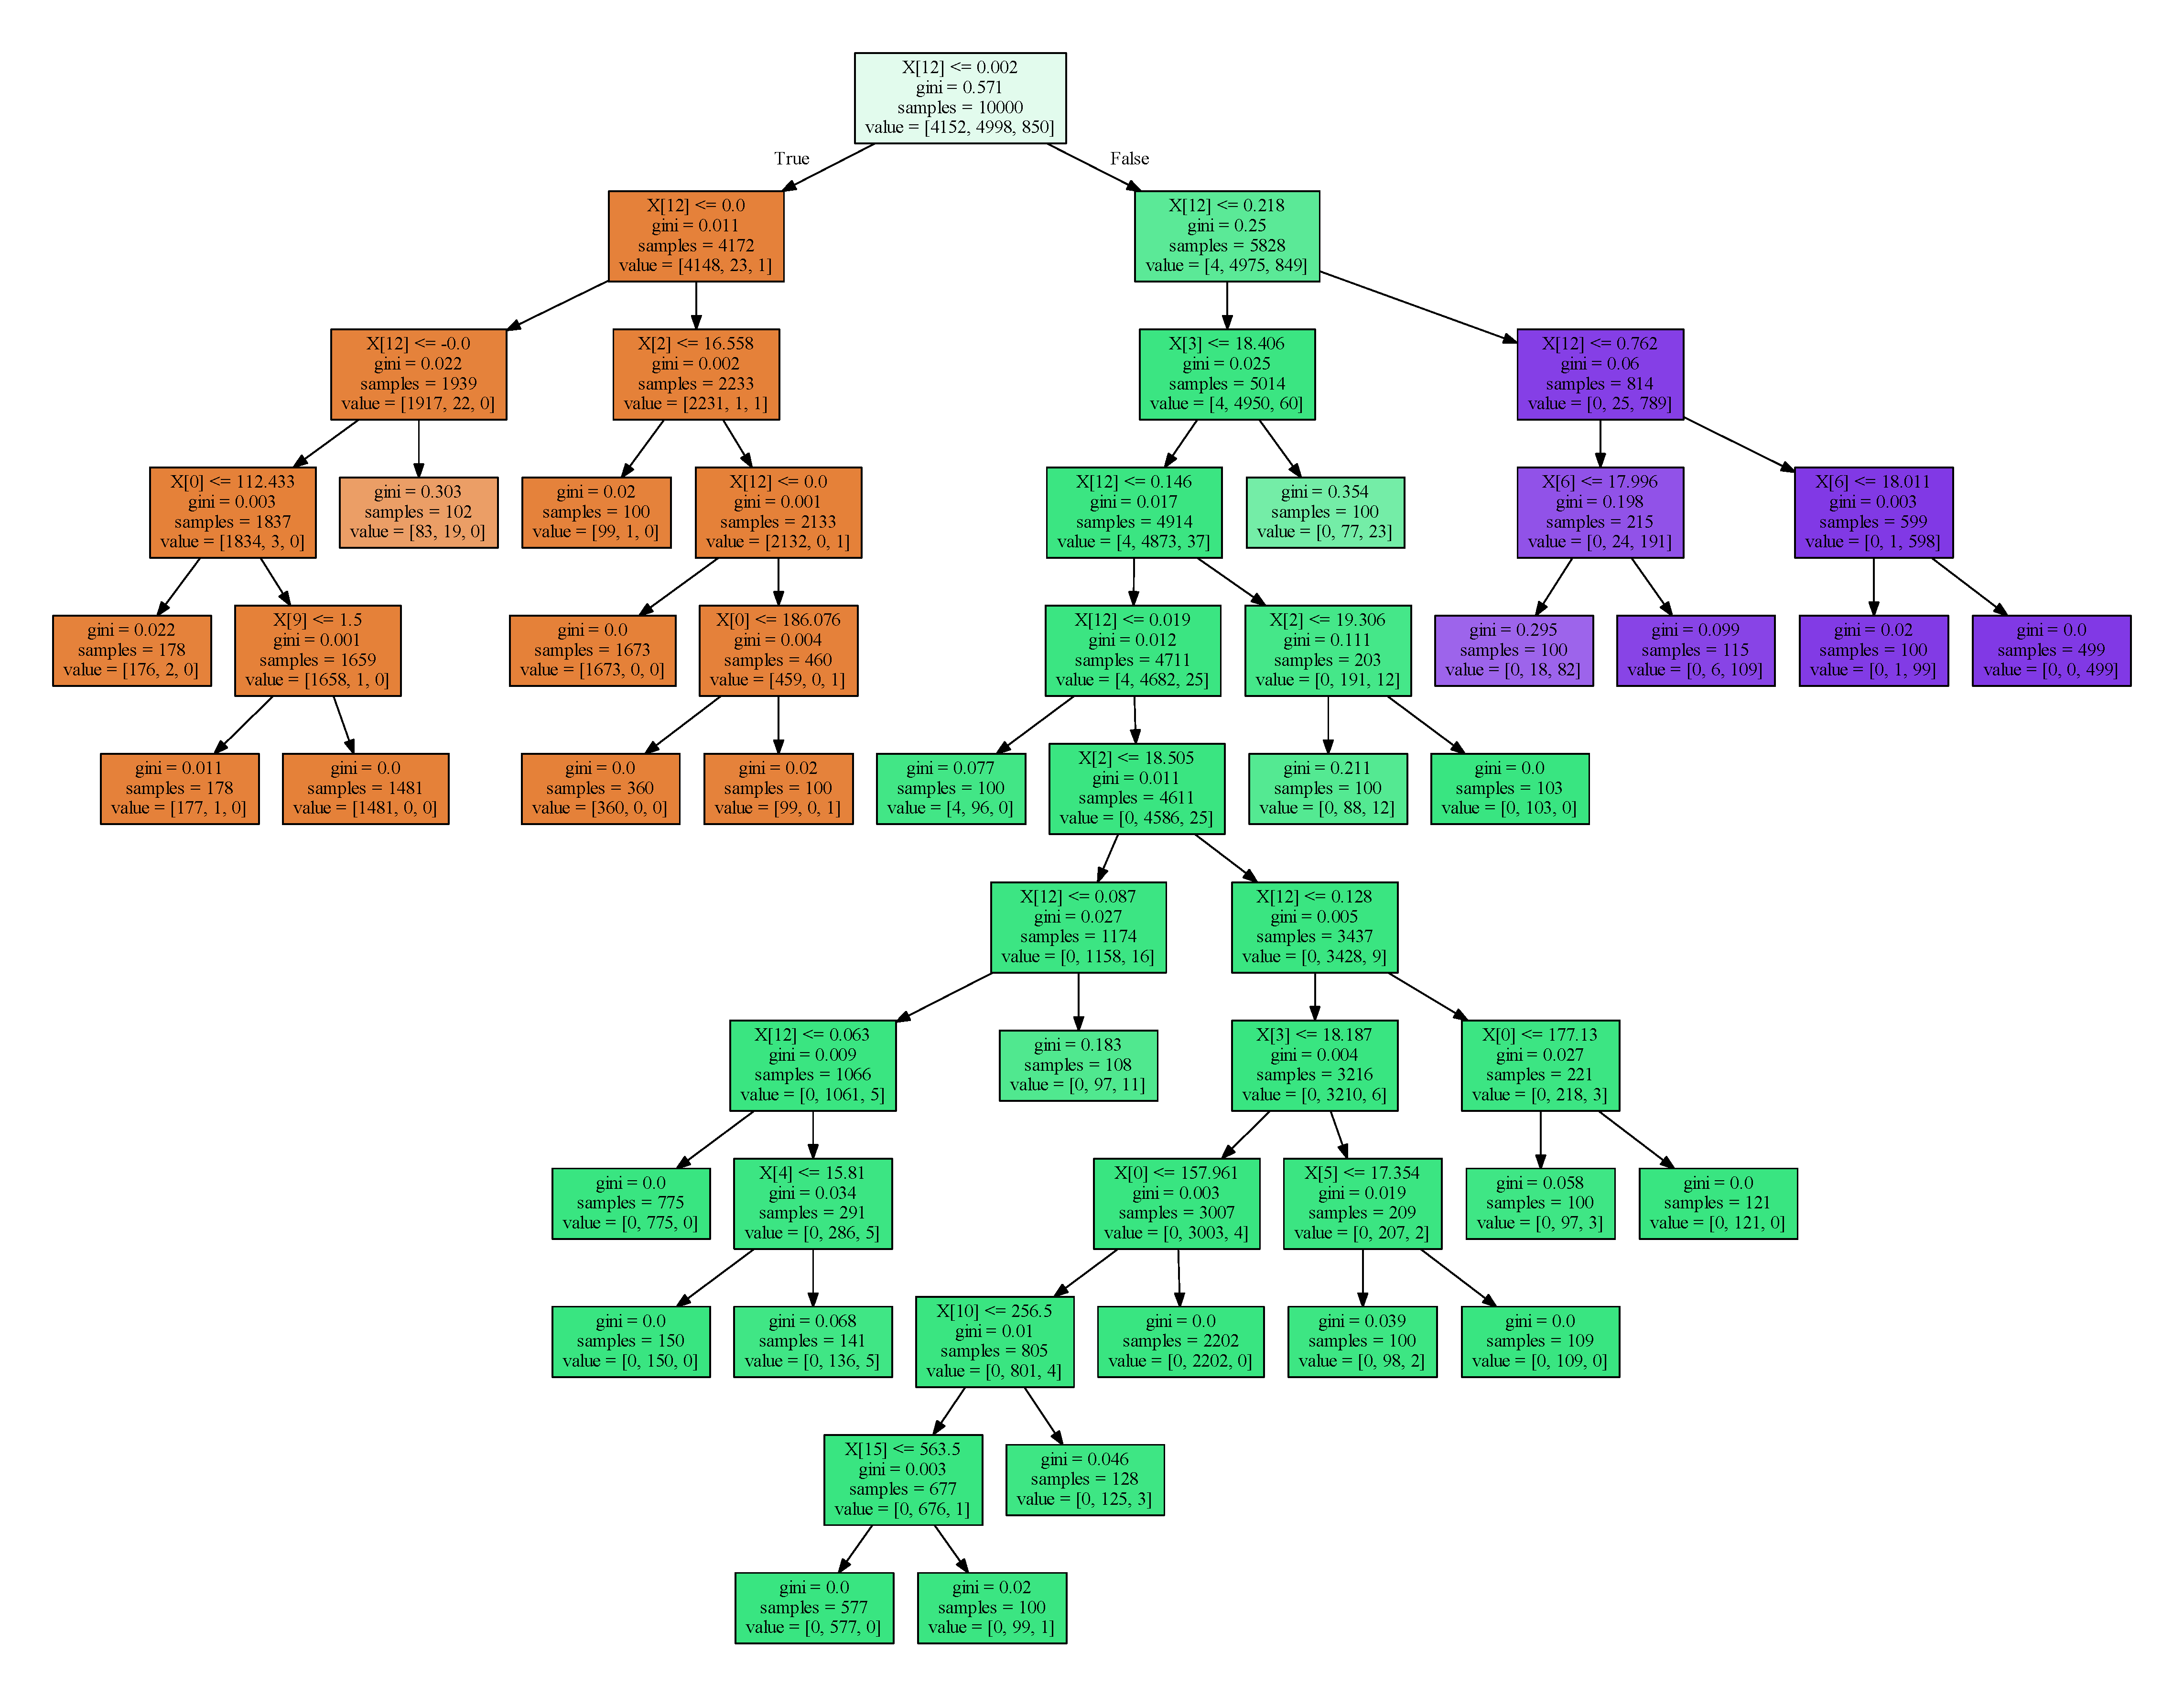
\includegraphics{img/Tree.png}
\caption{Tree}
\end{figure}

    \section{Question II The generalization
error}\label{question-ii-the-generalization-error}

    From the definition : \textgreater{} Gener. error = training error + 0.5
x \#of leaves

    We can write the code of calculate the generalization error like this:

    \begin{Verbatim}[commandchars=\\\{\}]
{\color{incolor}In [{\color{incolor}3}]:} \PY{c+c1}{\PYZsh{}Calculate the generalization error}
        \PY{n}{training\PYZus{}error} \PY{o}{=} \PY{p}{(}\PY{n+nb}{len}\PY{p}{(}\PY{n}{sky\PYZus{}class}\PY{p}{)} \PY{o}{\PYZhy{}} \PY{n}{clf}\PY{o}{.}\PY{n}{score}\PY{p}{(}\PY{n}{sky\PYZus{}data}\PY{p}{,}\PY{n}{sky\PYZus{}class}\PY{p}{)}\PY{o}{*}\PY{n+nb}{len}\PY{p}{(}\PY{n}{sky\PYZus{}class}\PY{p}{)}\PY{p}{)}\PY{o}{/}\PY{n+nb}{len}\PY{p}{(}\PY{n}{sky\PYZus{}class}\PY{p}{)}
        \PY{n}{array\PYZus{}children} \PY{o}{=} \PY{n}{clf}\PY{o}{.}\PY{n}{tree\PYZus{}}\PY{o}{.}\PY{n}{children\PYZus{}left}
        \PY{n}{num\PYZus{}leaves} \PY{o}{=} \PY{n}{np}\PY{o}{.}\PY{n}{count\PYZus{}nonzero}\PY{p}{(}\PY{n}{array\PYZus{}children} \PY{o}{==} \PY{o}{\PYZhy{}}\PY{l+m+mi}{1}\PY{p}{)}
        \PY{n}{gen\PYZus{}error} \PY{o}{=} \PY{n}{training\PYZus{}error} \PY{o}{+} \PY{p}{(}\PY{l+m+mf}{0.5}\PY{o}{*}\PY{n}{num\PYZus{}leaves}\PY{o}{/}\PY{n+nb}{len}\PY{p}{(}\PY{n}{sky\PYZus{}class}\PY{p}{)}\PY{p}{)}
        \PY{n+nb}{print}\PY{p}{(}\PY{l+s+s2}{\PYZdq{}}\PY{l+s+s2}{Training error: }\PY{l+s+s2}{\PYZdq{}}\PY{o}{+}\PY{n+nb}{str}\PY{p}{(}\PY{l+m+mi}{100}\PY{o}{*}\PY{n}{training\PYZus{}error}\PY{p}{)}\PY{o}{+}\PY{l+s+s2}{\PYZdq{}}\PY{l+s+s2}{\PYZpc{}}\PY{l+s+s2}{\PYZdq{}}\PY{p}{)}
        \PY{n+nb}{print}\PY{p}{(}\PY{l+s+s2}{\PYZdq{}}\PY{l+s+s2}{Number of nodes in the tree: }\PY{l+s+s2}{\PYZdq{}} \PY{o}{+}\PY{n+nb}{str}\PY{p}{(}\PY{n}{clf}\PY{o}{.}\PY{n}{tree\PYZus{}}\PY{o}{.}\PY{n}{node\PYZus{}count}\PY{p}{)}\PY{p}{)}
        \PY{n+nb}{print}\PY{p}{(}\PY{l+s+s1}{\PYZsq{}}\PY{l+s+s1}{Generalization error: }\PY{l+s+s1}{\PYZsq{}} \PY{o}{+} \PY{n+nb}{str}\PY{p}{(}\PY{l+m+mi}{100}\PY{o}{*}\PY{n}{gen\PYZus{}error}\PY{p}{)} \PY{o}{+} \PY{l+s+s1}{\PYZsq{}}\PY{l+s+s1}{\PYZpc{}}\PY{l+s+s1}{\PYZsq{}}\PY{p}{)}
\end{Verbatim}


    \begin{Verbatim}[commandchars=\\\{\}]
Training error: 1.13\%
Number of nodes in the tree: 55
Generalization error: 1.27\%

    \end{Verbatim}

    \section{Question III Change the
parameter}\label{question-iii-change-the-parameter}

    As we have seen in the results of the two precedent questions, the
training error we got is 1.13\%, which is near to the \emph{minimun
sample leafs} proportion we have chosen. If we observe the tree obtained
in question 1, we can see that after the second layer, because the
exceptions in each branch are less than 1\% of the total instances and
are distributed, which means they are not sufficient to become a leaf,
so that they are not successfully extracted.

So, we cannot reduce the training error by pre-pruning the data with the
parameters of this classifer, what we can do in order to minimize the
number of leaves is to cut as many leaves as possible without changing
the classification result. If we observe the tree generated in the first
question, we can see that we can cut all the nodes in the left branch up
to the first layer, and the right branch up to the second layer.

For achieving this, we can simply set \textbf{\emph{max\_leaf\_node =
3}}, this will minimize the leafs cause we need at least three nodes for
three possible class and in the tree of question 1, no new significant
division is generated from the first three nodes.

the code, the result is shown below:

    \begin{Verbatim}[commandchars=\\\{\}]
{\color{incolor}In [{\color{incolor}38}]:} \PY{c+c1}{\PYZsh{}Load the data and training}
         \PY{n}{clf} \PY{o}{=} \PY{n}{tree}\PY{o}{.}\PY{n}{DecisionTreeClassifier}\PY{p}{(}\PY{n}{min\PYZus{}samples\PYZus{}leaf}\PY{o}{=}\PY{l+m+mf}{0.01}\PY{p}{,} \PY{n}{max\PYZus{}leaf\PYZus{}nodes} \PY{o}{=} \PY{l+m+mi}{3}\PY{p}{)}
         \PY{n}{clf}\PY{o}{.}\PY{n}{fit}\PY{p}{(}\PY{n}{sky\PYZus{}data}\PY{p}{,} \PY{n}{sky\PYZus{}class}\PY{p}{)}
         
         \PY{c+c1}{\PYZsh{}Draw the tree into a pdf}
         \PY{n}{dot\PYZus{}data} \PY{o}{=} \PY{n}{StringIO}\PY{p}{(}\PY{p}{)}
         \PY{n}{tree}\PY{o}{.}\PY{n}{export\PYZus{}graphviz}\PY{p}{(}\PY{n}{clf}\PY{p}{,} \PY{n}{out\PYZus{}file}\PY{o}{=}\PY{n}{dot\PYZus{}data}\PY{p}{,} \PY{n}{filled}\PY{o}{=}\PY{k+kc}{True}\PY{p}{)}
         \PY{n}{graph} \PY{o}{=} \PY{n}{pydotplus}\PY{o}{.}\PY{n}{graph\PYZus{}from\PYZus{}dot\PYZus{}data}\PY{p}{(}\PY{n}{dot\PYZus{}data}\PY{o}{.}\PY{n}{getvalue}\PY{p}{(}\PY{p}{)}\PY{p}{)}
         \PY{n}{graph}\PY{o}{.}\PY{n}{write\PYZus{}pdf}\PY{p}{(}\PY{l+s+s2}{\PYZdq{}}\PY{l+s+s2}{Tree\PYZus{}modified.pdf}\PY{l+s+s2}{\PYZdq{}}\PY{p}{)}
         
         \PY{c+c1}{\PYZsh{}Calculate the generalization error}
         \PY{n}{training\PYZus{}error} \PY{o}{=} \PY{p}{(}\PY{n+nb}{len}\PY{p}{(}\PY{n}{sky\PYZus{}class}\PY{p}{)} \PY{o}{\PYZhy{}} \PY{n}{clf}\PY{o}{.}\PY{n}{score}\PY{p}{(}\PY{n}{sky\PYZus{}data}\PY{p}{,}\PY{n}{sky\PYZus{}class}\PY{p}{)}\PY{o}{*}\PY{n+nb}{len}\PY{p}{(}\PY{n}{sky\PYZus{}class}\PY{p}{)}\PY{p}{)}\PY{o}{/}\PY{n+nb}{len}\PY{p}{(}\PY{n}{sky\PYZus{}class}\PY{p}{)}
         \PY{n}{array\PYZus{}children} \PY{o}{=} \PY{n}{clf}\PY{o}{.}\PY{n}{tree\PYZus{}}\PY{o}{.}\PY{n}{children\PYZus{}left}
         \PY{n}{num\PYZus{}leaves} \PY{o}{=} \PY{n}{np}\PY{o}{.}\PY{n}{count\PYZus{}nonzero}\PY{p}{(}\PY{n}{array\PYZus{}children} \PY{o}{==} \PY{o}{\PYZhy{}}\PY{l+m+mi}{1}\PY{p}{)}
         \PY{n}{gen\PYZus{}error} \PY{o}{=} \PY{n}{training\PYZus{}error} \PY{o}{+} \PY{p}{(}\PY{l+m+mf}{0.5}\PY{o}{*}\PY{n}{num\PYZus{}leaves}\PY{o}{/}\PY{n+nb}{len}\PY{p}{(}\PY{n}{sky\PYZus{}class}\PY{p}{)}\PY{p}{)}
         \PY{n+nb}{print}\PY{p}{(}\PY{l+s+s1}{\PYZsq{}}\PY{l+s+s1}{Training error: }\PY{l+s+s1}{\PYZsq{}} \PY{o}{+} \PY{n+nb}{str}\PY{p}{(}\PY{l+m+mi}{100}\PY{o}{*}\PY{n}{training\PYZus{}error}\PY{p}{)} \PY{o}{+} \PY{l+s+s1}{\PYZsq{}}\PY{l+s+s1}{\PYZpc{}}\PY{l+s+s1}{\PYZsq{}}\PY{p}{)}
         \PY{n+nb}{print}\PY{p}{(}\PY{l+s+s1}{\PYZsq{}}\PY{l+s+s1}{Number of leaves: }\PY{l+s+s1}{\PYZsq{}} \PY{o}{+} \PY{n+nb}{str}\PY{p}{(}\PY{n}{num\PYZus{}leaves}\PY{p}{)}\PY{p}{)}
         \PY{n+nb}{print}\PY{p}{(}\PY{l+s+s1}{\PYZsq{}}\PY{l+s+s1}{Generalization error: }\PY{l+s+s1}{\PYZsq{}} \PY{o}{+} \PY{n+nb}{str}\PY{p}{(}\PY{l+m+mi}{100}\PY{o}{*}\PY{n}{gen\PYZus{}error}\PY{p}{)} \PY{o}{+} \PY{l+s+s1}{\PYZsq{}}\PY{l+s+s1}{\PYZpc{}}\PY{l+s+s1}{\PYZsq{}}\PY{p}{)}
\end{Verbatim}


    \begin{Verbatim}[commandchars=\\\{\}]
Training error: 1.13\%
Number of leaves: 3
Generalization error: 1.145\%

    \end{Verbatim}

    We can see that the training error has not changed even if we has set
the number of leaves to 3, the minimum value possible for this case. Yet
another way to has a tree like this is to set
\textbf{\emph{min\_impurity\_decrease=t}}, where \textbf{\emph{t}} is a
value big enough to prevent the second spilt in the left main branch but
no too big to cease the spilt in the right branch. Amd we can also set
\emph{t} in a value that can exactly give us the three leaves tree we
need, this is possible because except the three splits , all other spilt
will just decrease the impurity a very little bit, any value between
\textbf{\emph{0.01(1\%, the minimum sample leafs)}} and
\textbf{\emph{0.113(1.13\%, the training error)}} will do (\textbf{En
effet, the real range will be wider than this, but the calculation of
the exact range is pointless}).

Or, more simply, we can add \emph{max\_depth=2}, and use a very samll
value of \emph{t}, because the split in the leaf has just decreased the
impurity for a negligible amount. For instance,
\textbf{\emph{max\_depth=2, min\_impurity\_decrease=0.00003}} will do.

Below is the tree obtained in these three ways.

    \begin{figure}
\centering
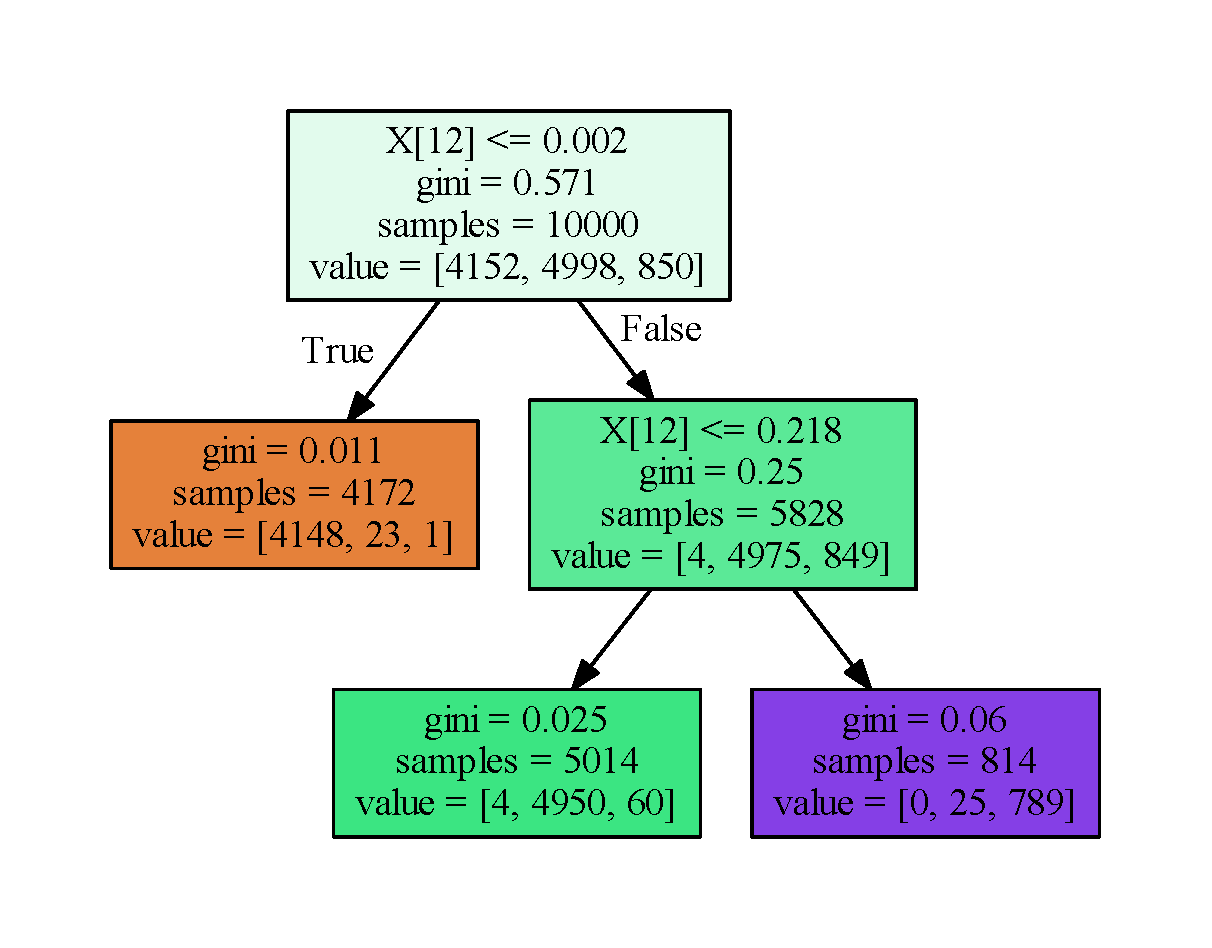
\includegraphics{img/Tree_modified.png}
\caption{Tree Modified}
\end{figure}

    \section{Question IV Comparison}\label{question-iv-comparison}

    The answer is direct, I will choose \textbf{the best one I obtained in
point 2}, If the final classification result is the same, we do not need
to perform the following classification procedures, the latter tree will
deliver the same result, but just in two comparisons in maximum.

    \section{Question V Insights}\label{question-v-insights}

    \begin{Verbatim}[commandchars=\\\{\}]
{\color{incolor}In [{\color{incolor}39}]:} \PY{n}{three\PYZus{}object} \PY{o}{=} \PY{n}{np}\PY{o}{.}\PY{n}{array}\PY{p}{(}\PY{p}{[}\PY{p}{[}\PY{l+m+mi}{199}\PY{p}{,} \PY{l+m+mf}{0.2}\PY{p}{,} \PY{l+m+mi}{19}\PY{p}{,} \PY{l+m+mi}{18}\PY{p}{,} \PY{l+m+mi}{18}\PY{p}{,} \PY{l+m+mi}{18}\PY{p}{,} \PY{l+m+mi}{16}\PY{p}{,} \PY{l+m+mi}{777}\PY{p}{,} \PY{l+m+mi}{301}\PY{p}{,} \PY{l+m+mf}{3.0}\PY{p}{,} \PY{l+m+mi}{270}\PY{p}{,} \PY{l+m+mf}{3.312}\PY{p}{,} \PY{l+m+mf}{0.001}\PY{p}{,} \PY{l+m+mi}{288}\PY{p}{,} \PY{l+m+mi}{51739}\PY{p}{,} \PY{l+m+mi}{550}\PY{p}{]}\PY{p}{,}
                                \PY{p}{[}\PY{l+m+mi}{199}\PY{p}{,} \PY{l+m+mf}{0.2}\PY{p}{,} \PY{l+m+mi}{19}\PY{p}{,} \PY{l+m+mi}{18}\PY{p}{,} \PY{l+m+mi}{18}\PY{p}{,} \PY{l+m+mi}{18}\PY{p}{,} \PY{l+m+mi}{16}\PY{p}{,} \PY{l+m+mi}{777}\PY{p}{,} \PY{l+m+mi}{301}\PY{p}{,} \PY{l+m+mf}{3.0}\PY{p}{,} \PY{l+m+mi}{270}\PY{p}{,} \PY{l+m+mf}{3.312}\PY{p}{,} \PY{l+m+mf}{0.119}\PY{p}{,} \PY{l+m+mi}{288}\PY{p}{,} \PY{l+m+mi}{51739}\PY{p}{,} \PY{l+m+mi}{550}\PY{p}{]}\PY{p}{,}
                                \PY{p}{[}\PY{l+m+mi}{199}\PY{p}{,} \PY{l+m+mf}{0.2}\PY{p}{,} \PY{l+m+mi}{19}\PY{p}{,} \PY{l+m+mi}{18}\PY{p}{,} \PY{l+m+mi}{18}\PY{p}{,} \PY{l+m+mi}{18}\PY{p}{,} \PY{l+m+mi}{16}\PY{p}{,} \PY{l+m+mi}{777}\PY{p}{,} \PY{l+m+mi}{301}\PY{p}{,} \PY{l+m+mf}{3.0}\PY{p}{,} \PY{l+m+mi}{270}\PY{p}{,} \PY{l+m+mf}{3.312}\PY{p}{,} \PY{l+m+mf}{0.219}\PY{p}{,} \PY{l+m+mi}{288}\PY{p}{,} \PY{l+m+mi}{51739}\PY{p}{,} \PY{l+m+mi}{550}\PY{p}{]}\PY{p}{]}\PY{p}{)}
         \PY{n}{Class\PYZus{}value} \PY{o}{=} \PY{n}{clf}\PY{o}{.}\PY{n}{predict}\PY{p}{(}\PY{n}{three\PYZus{}object}\PY{p}{)}
         \PY{n+nb}{print}\PY{p}{(}\PY{n}{Class\PYZus{}value}\PY{p}{)}
\end{Verbatim}


    \begin{Verbatim}[commandchars=\\\{\}]
[0. 1. 2.]

    \end{Verbatim}

    For this test, I have constructed three objects which carry the exact
same data except the differences in \textbf{X{[}12{]}}, which is the
\textbf{"Final Redshift"} of the sky object, but we have seen that the
three object are successsfully classified.

The \textbf{insights} for this tree need to be discussed in two aspects.
\textbf{On one hand}, if a 1.145\% error rate is acceptable, we can
conclude that only the redshift feature is enough to distinguish stars,
galaxies and Quasars so that we can use it as a criterion, or at least
we can say that the redshift is the main difference between these three
categories. \textbf{On the other hand}, a 1.145\% error rate is still a
little high, and this tree is even kind of robust because all the other
features haven't been used, we can still get the result from the
redshift no matter how ridiculous the other features are. But we have to
admit that by \emph{pruning} like this, we do have minimized the
generalization error.

Consequently, it will be kind of a dilemma if we can neither accept an
error over 1\% nor simply take redshift as a criterion. However in fact
an error that is just a little larger than 1\% is quite normal with the
minimum sample numbers for a leaf being 1\% of total instances, this
tree don't have problems like \emph{underfitting} or \emph{overfitting}
to this extent.

    \section{Question VI Post-pruning or not
?}\label{question-vi-post-pruning-or-not}

    The answer is no. Now I only have three leaves and three classes to
classify in the meantime, thus it is not possible to perform further
pruning. Any further pruning will cause a whole class of instances to be
misplaced, which will greatly increase the training error.

    \section{Question VII The implement of
post-pruning}\label{question-vii-the-implement-of-post-pruning}

    I have implemented the post-pruning policy like this. But on top of what
we have discussed in the precedent questions, I choose to \textbf{add an
Exception} to throw when the tree got in can no longer be pruned. When
the tree can be pruned, in this case, I have firstly caculated the
misplaced instances in a node, if the number of misplaced instances in
this node is smaller than the minimum requirement for a leaf, we can cut
it because it will either not increase the training error, or increase
the error by a amount less than 0.5 x \#leaves\_cutted, which will in
turn \textbf{reduce the generalization error}.

    \begin{Verbatim}[commandchars=\\\{\}]
{\color{incolor}In [{\color{incolor}55}]:} \PY{k}{def} \PY{n+nf}{post\PYZus{}pruning}\PY{p}{(}\PY{n}{tree}\PY{p}{)}\PY{p}{:}
             \PY{n}{min\PYZus{}leaf} \PY{o}{=} \PY{l+m+mi}{1}
             \PY{n}{tempm} \PY{o}{=} \PY{n}{tree}\PY{o}{.}\PY{n}{min\PYZus{}samples\PYZus{}leaf}
             \PY{k}{if} \PY{n}{tempm} \PY{o}{!=} \PY{k+kc}{None}\PY{p}{:}
                 \PY{k}{if} \PY{n}{tempm} \PY{o}{\PYZlt{}} \PY{l+m+mi}{1}\PY{p}{:}
                     \PY{n}{min\PYZus{}leaf} \PY{o}{=} \PY{n}{tempm} \PY{o}{*} \PY{n}{clf}\PY{o}{.}\PY{n}{tree\PYZus{}}\PY{o}{.}\PY{n}{n\PYZus{}node\PYZus{}samples}\PY{p}{[}\PY{l+m+mi}{0}\PY{p}{]}
                 \PY{k}{if} \PY{n}{tempm} \PY{o}{\PYZgt{}} \PY{l+m+mi}{1}\PY{p}{:}
                     \PY{n}{min\PYZus{}leaf} \PY{o}{=} \PY{n}{tempm}    
             \PY{n}{array\PYZus{}children} \PY{o}{=} \PY{n}{tree}\PY{o}{.}\PY{n}{tree\PYZus{}}\PY{o}{.}\PY{n}{children\PYZus{}left}
             \PY{n}{num\PYZus{}leaves} \PY{o}{=} \PY{n}{np}\PY{o}{.}\PY{n}{count\PYZus{}nonzero}\PY{p}{(}\PY{n}{array\PYZus{}children} \PY{o}{==} \PY{o}{\PYZhy{}}\PY{l+m+mi}{1}\PY{p}{)}
             \PY{n}{n} \PY{o}{=} \PY{n}{tree}\PY{o}{.}\PY{n}{n\PYZus{}classes\PYZus{}}
             \PY{k}{if} \PY{n}{n} \PY{o}{\PYZgt{}}\PY{o}{=} \PY{n}{num\PYZus{}leaves}\PY{p}{:}
                 \PY{k}{raise} \PY{n+ne}{Exception}\PY{p}{(}\PY{l+s+s1}{\PYZsq{}}\PY{l+s+s1}{Tree can no longer be pruned.}\PY{l+s+s1}{\PYZsq{}}\PY{p}{)}
             \PY{k}{else}\PY{p}{:}
                 \PY{k}{for} \PY{n}{i} \PY{o+ow}{in} \PY{n+nb}{range}\PY{p}{(}\PY{n}{tree}\PY{o}{.}\PY{n}{tree\PYZus{}}\PY{o}{.}\PY{n}{node\PYZus{}count}\PY{p}{)}\PY{p}{:}
                     \PY{n}{values} \PY{o}{=} \PY{n}{tree}\PY{o}{.}\PY{n}{tree\PYZus{}}\PY{o}{.}\PY{n}{value}\PY{p}{[}\PY{n}{i}\PY{p}{,}\PY{l+m+mi}{0}\PY{p}{]}
                     \PY{n}{instance\PYZus{}misplaced} \PY{o}{=} \PY{n+nb}{sum}\PY{p}{(}\PY{n}{values}\PY{p}{)}\PY{o}{\PYZhy{}}\PY{n+nb}{max}\PY{p}{(}\PY{n}{values}\PY{p}{)}
                     \PY{k}{if} \PY{n}{instance\PYZus{}misplaced} \PY{o}{\PYZlt{}} \PY{n}{min\PYZus{}leaf}\PY{p}{:}
                         \PY{n}{tree}\PY{o}{.}\PY{n}{tree\PYZus{}}\PY{o}{.}\PY{n}{children\PYZus{}left}\PY{p}{[}\PY{n}{i}\PY{p}{]} \PY{o}{=} \PY{o}{\PYZhy{}}\PY{l+m+mi}{1}
                         \PY{n}{tree}\PY{o}{.}\PY{n}{tree\PYZus{}}\PY{o}{.}\PY{n}{children\PYZus{}right}\PY{p}{[}\PY{n}{i}\PY{p}{]} \PY{o}{=} \PY{o}{\PYZhy{}}\PY{l+m+mi}{1}
         
         \PY{n}{post\PYZus{}pruning}\PY{p}{(}\PY{n}{clf}\PY{p}{)}
         
         \PY{n}{dot\PYZus{}data} \PY{o}{=} \PY{n}{StringIO}\PY{p}{(}\PY{p}{)}
         \PY{n}{tree}\PY{o}{.}\PY{n}{export\PYZus{}graphviz}\PY{p}{(}\PY{n}{clf}\PY{p}{,} \PY{n}{out\PYZus{}file}\PY{o}{=}\PY{n}{dot\PYZus{}data}\PY{p}{,} \PY{n}{filled}\PY{o}{=} \PY{k+kc}{True}\PY{p}{)}
         \PY{n}{graph} \PY{o}{=} \PY{n}{pydotplus}\PY{o}{.}\PY{n}{graph\PYZus{}from\PYZus{}dot\PYZus{}data}\PY{p}{(}\PY{n}{dot\PYZus{}data}\PY{o}{.}\PY{n}{getvalue}\PY{p}{(}\PY{p}{)}\PY{p}{)}
         \PY{n}{graph}\PY{o}{.}\PY{n}{write\PYZus{}pdf}\PY{p}{(}\PY{l+s+s2}{\PYZdq{}}\PY{l+s+s2}{Tree\PYZus{}pruned.pdf}\PY{l+s+s2}{\PYZdq{}}\PY{p}{)}
\end{Verbatim}


    \begin{Verbatim}[commandchars=\\\{\}]

        ---------------------------------------------------------------------------

        Exception                                 Traceback (most recent call last)

        <ipython-input-55-576f7ac0de04> in <module>()
         20                 tree.tree\_.children\_right[i] = -1
         21 
    ---> 22 post\_pruning(clf)
    

        <ipython-input-55-576f7ac0de04> in post\_pruning(tree)
         11     n = tree.n\_classes\_
         12     if n >= num\_leaves:
    ---> 13         raise Exception('Tree can no longer be pruned.')
         14     else:
         15         for i in range(tree.tree\_.node\_count):
    

        Exception: Tree can no longer be pruned.

    \end{Verbatim}

    From the result above we can see that, this funtion returned the
exception as expected for the \textbf{best tree in point 2}, But if we
test this function with the tree we got from the default configuration,
alias \textbf{the tree in point 1}, we can get a tree same as the best
tree in point 2, which means this function works.


    % Add a bibliography block to the postdoc
    
    
    
    \end{document}
